\chapter{Core Systems Design}
\label{cha:core_system_design}
\section{Requirements Analysis}
\subsection{User Requirements}
The following user requirements for the system were gathered by inspecting similar systems, personal creativity and feedback from supervisor or wearables lab team. User stories were chosen for representation: \ref{table:userStories}.
\begin{center}
        \begin{longtblr}[
            caption={User Stories},
            label={table:userStories}
        ] {
            colspec = {|X|X|},
            rowhead = 1,
            hlines,
        }

        User Story & Acceptance Criteria  \\ 

        As a user I can view health data originating from Oura and Withings devices on a single central dashboard UI, so that I can quickly compare measurements between the devices and also manually examine my physical activity and sleep trends.
        & 
        Given that user is authenticated, when the user is on the dashboard page, the dashboard is displayed, containing a graph visualising last 7 days of data from both devices, with each line colored differently for each device; also buttons to switch which property, such as steps per day, should be displayed on the graph.
        \\ 

        As a user I can download all of my data as a csv file by pressing a button in the UI, so that I have my personal data conveniently in one file, in a widely supported format, which could be used for backing-up my data tp other storage solution, running data analysis etc.
        & 
        Given that user is authenticated, when the user presses 'Export CSV' button on the main page's UI, the csv file download starts, with that file containing all of the health measurements data persisted in the system's database at that time 
        \\ 

        As a user I can critically reflect on the passed day, with helpful insights and data presented on the UI; I also want to be reminded about this everyday at a certain configurable time; So that I can assess my progress towards my health goals, take pride in my accomplishments today and identify areas to improve on tomorrow.
        & 
        Given that user is authenticated, at a user configured time, the user is notified about daily report being available. On the daily report UI page, there is feedback highlighting areas of achievement and areas to improve on; as well as a graph visualising user's progress towards their weekly activity goals, as well as how well/poor the predicted daily activity norm was achieved
        \\

        As a user I can critically reflect on the passed week, with helpful insights and data presented on the UI; I also want to be reminded about this everyday at a certain configurable time; So that I can assess my consistency in physical activity or sleep, as well as compare this with the previous week.
        &
        Given that user is authenticated, when the user configured time is reached, the user is notified about weekly report being available. On the weekly report UI page, there are graphs visualising consistency in key metrics of MET minutes and sleep score; as well as numerical value quantifying the consistency, with a comparison to the 3 previous weeks. 
       \\

       As a user I want to receive activity reminders throughout the day at configurable times containing a list of curated exercises, with description and video example on how to perform them, that are well suited to my preferences and health data so far in the week; So that I am encouraged to fullfil my weekly activity goals; saving time by not having to create a good exercise regiment myself or saving money by not paying somebody else to do it.  
       &
       Given that the user is authenticated, when the user configured time is reached, the user is notified about daily exercise. On the exercises UI page, there is achieved to expected activity counter and curated list of exercises, which respect the following user configured preferences: athleticism level, MET weekly target, excluded activities, gym days and home equipment; as well as taking gathered health data into consideration.
       \\
       As a user I can submit free-form natural language questions and then receive natural language answers, which should be influenced as required by my health data and my profile; accessible though UI. So that I can have natural conversation about my health like I would with a real-life personal trainer, providing guidance and sense of not being alone.
       &
       Given that the user is authenticated, when the user visits the the AI Chat UI page there is a chat containing past user's requests and system's responses; there is an input box where the user can type a question using natural language. After submitting the question a reply is sent, which takes into account user's health data and their profile.

        \end{longtblr}
    \end{center}

\subsection{Functional Requirements}
The following functional requirements were derived so that user requirements could be fulfilled. System use case UML diagram, Flowchart and textual descriptions were used as representations.
\begin{itemize}
    \item Sync and view data diagram: \ref{fig:2}
    \item Export data diagram: \ref{fig:3}
    \item Daily \& Weekly Reports diagram: \ref{fig:4}
    \item AI Inference flowchart: \ref{fig:5}
    \item Activity Plan diagram: \ref{fig:6}
    \item Personalisation: User is able to configure their profile, which is saved in the database and used to customise modifiable parameters of the system. The profile has the following fields: 
    \begin{itemize}
        \item Height in Cm: Integer
        \item Weight in Kg: Integer
        \item MET Minutes weekly target: Integer
        \item Excluded Activity Keywords List of strings
        \item Athleticism: Enum [Beginner, Intermediate, Expert]
        \item Gym Days: List of Days of the week
        \item Home equipment: List of strings
        \item Report notification time: Time
        \item Daily Activity Reminder times: List of Times
    \end{itemize}
\end{itemize}
\begin{figure}
    
    \centering
    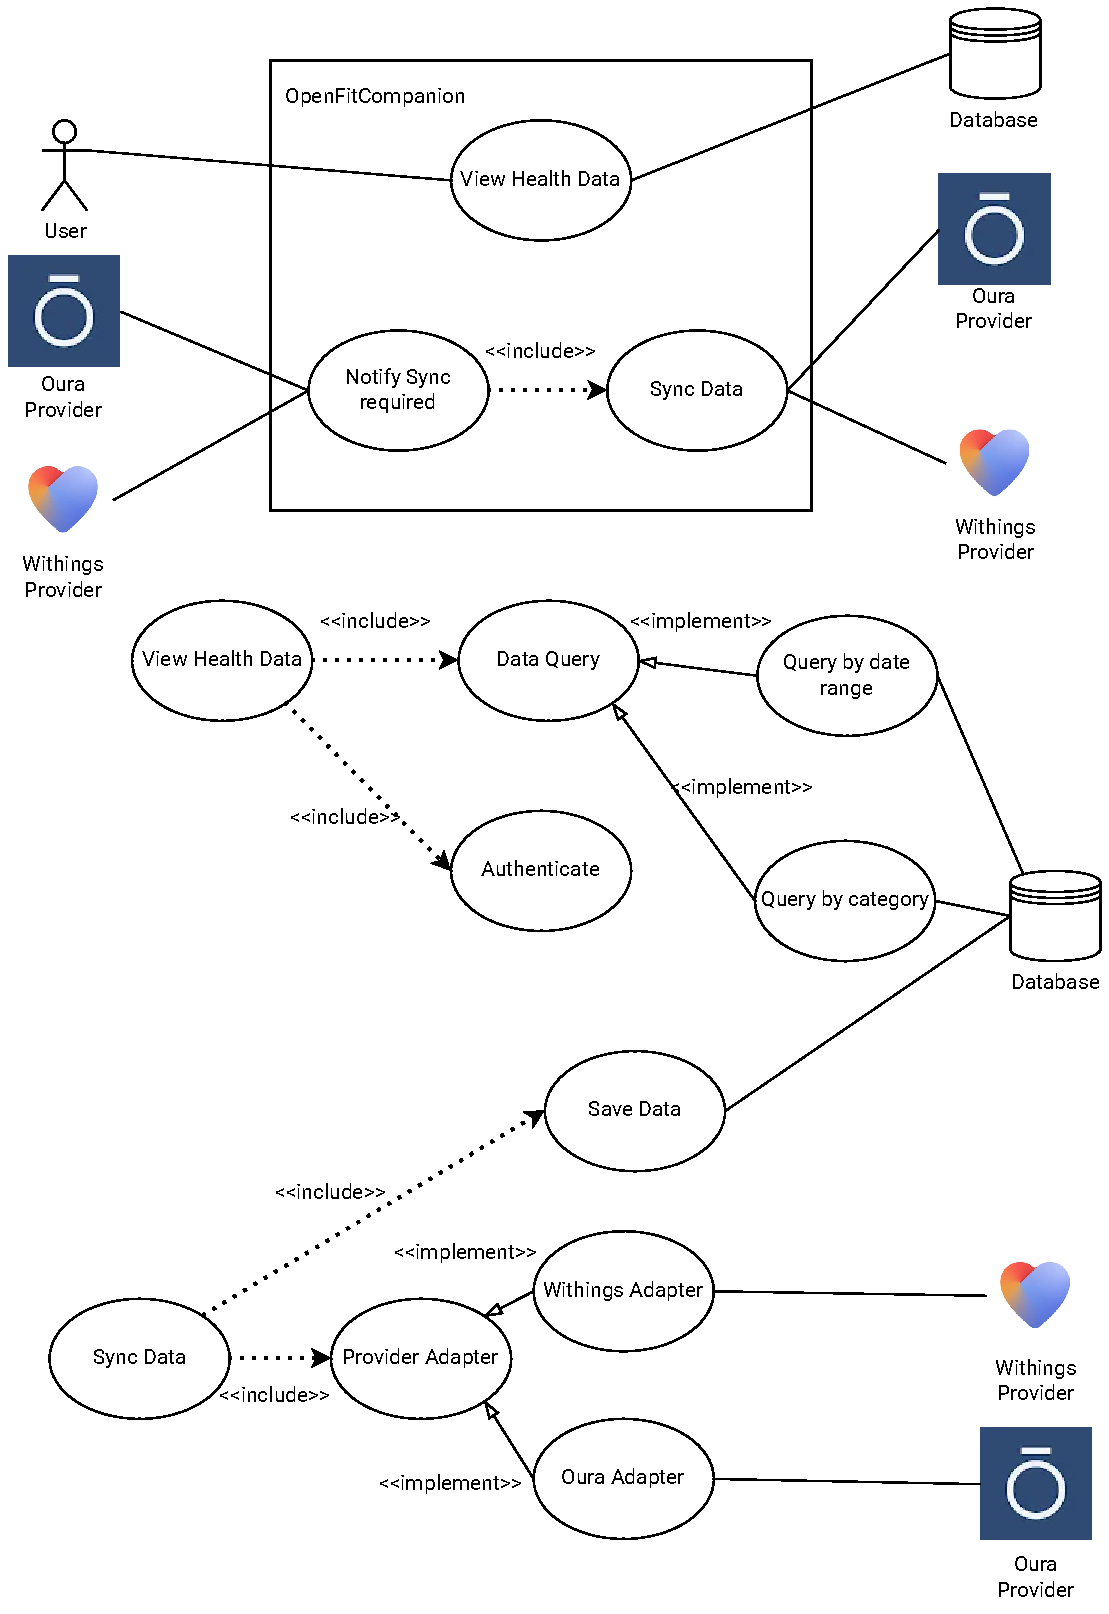
\includegraphics[width=\textwidth,height=\textheight,keepaspectratio]{../images/viewFunc.pdf}
    \caption{View data use case UML diagram}
    \label{fig:2}
\end{figure}
\begin{figure}
    
    \centering
    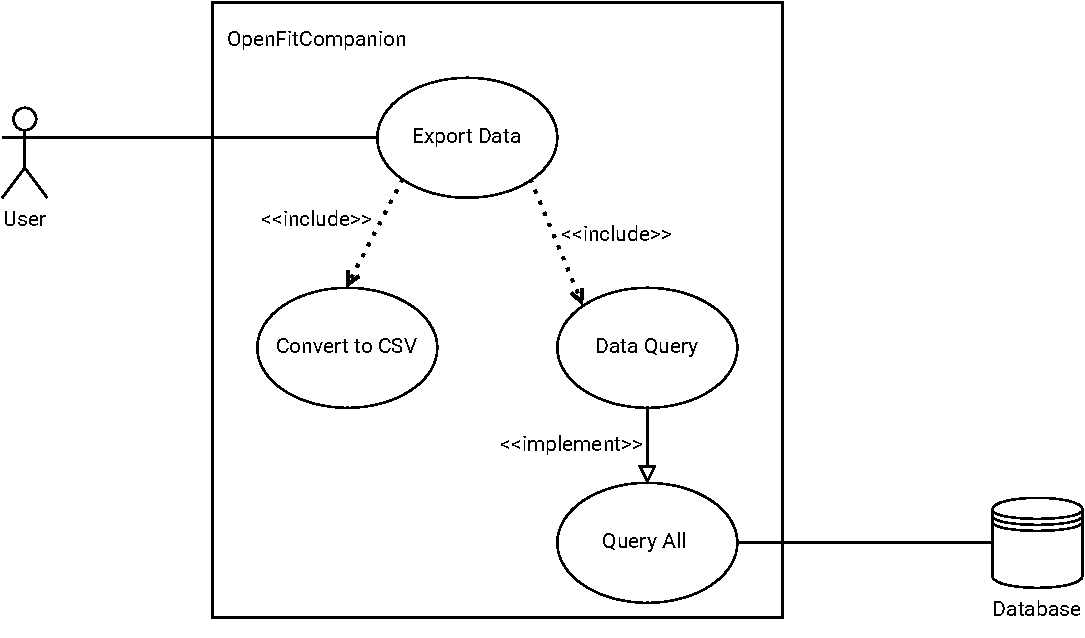
\includegraphics[width=\textwidth,height=\textheight,keepaspectratio]{../images/exportDataFunc.pdf}
    \caption{Export data use case UML diagram}
    \label{fig:3}
    
\end{figure}
\begin{figure}
    
    \centering
    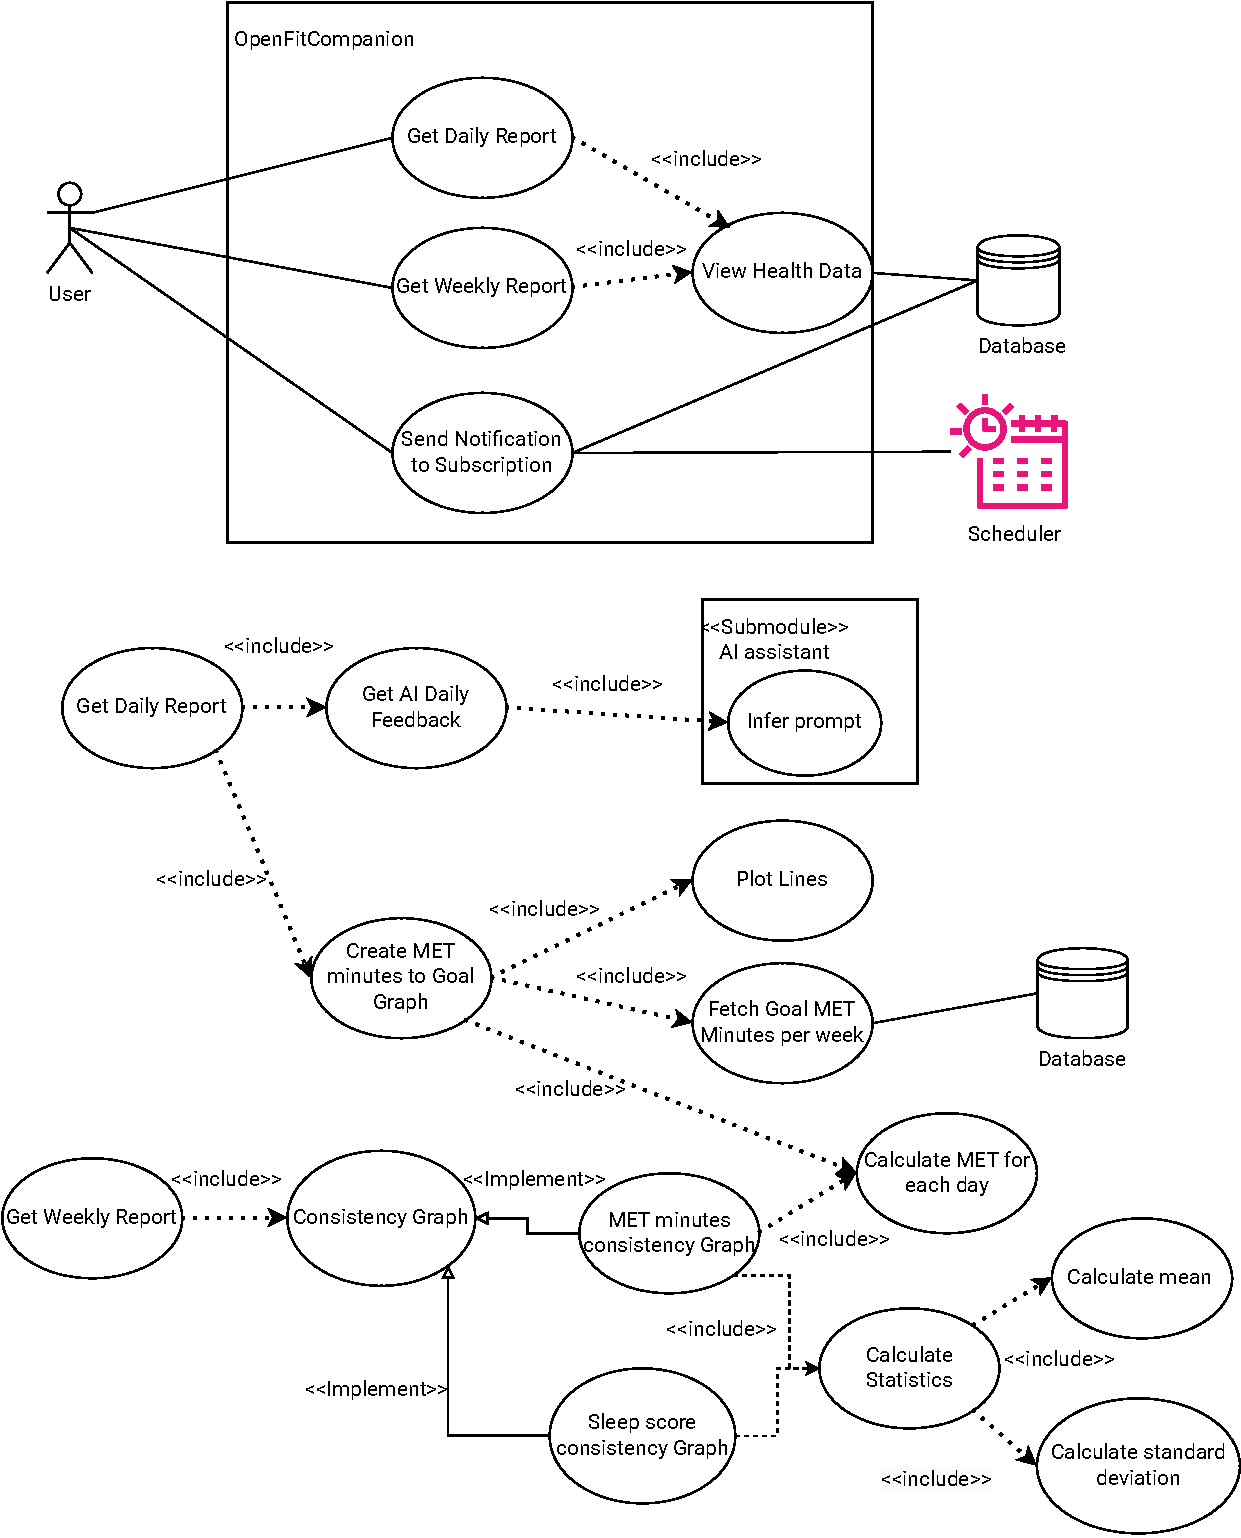
\includegraphics[width=\textwidth,height=\textheight,keepaspectratio]{../images/reports.pdf}
    \caption{Daily \& Weekly Reports use case UML diagram}
    \label{fig:4}
    
\end{figure}
\begin{figure}
    
    \centering
    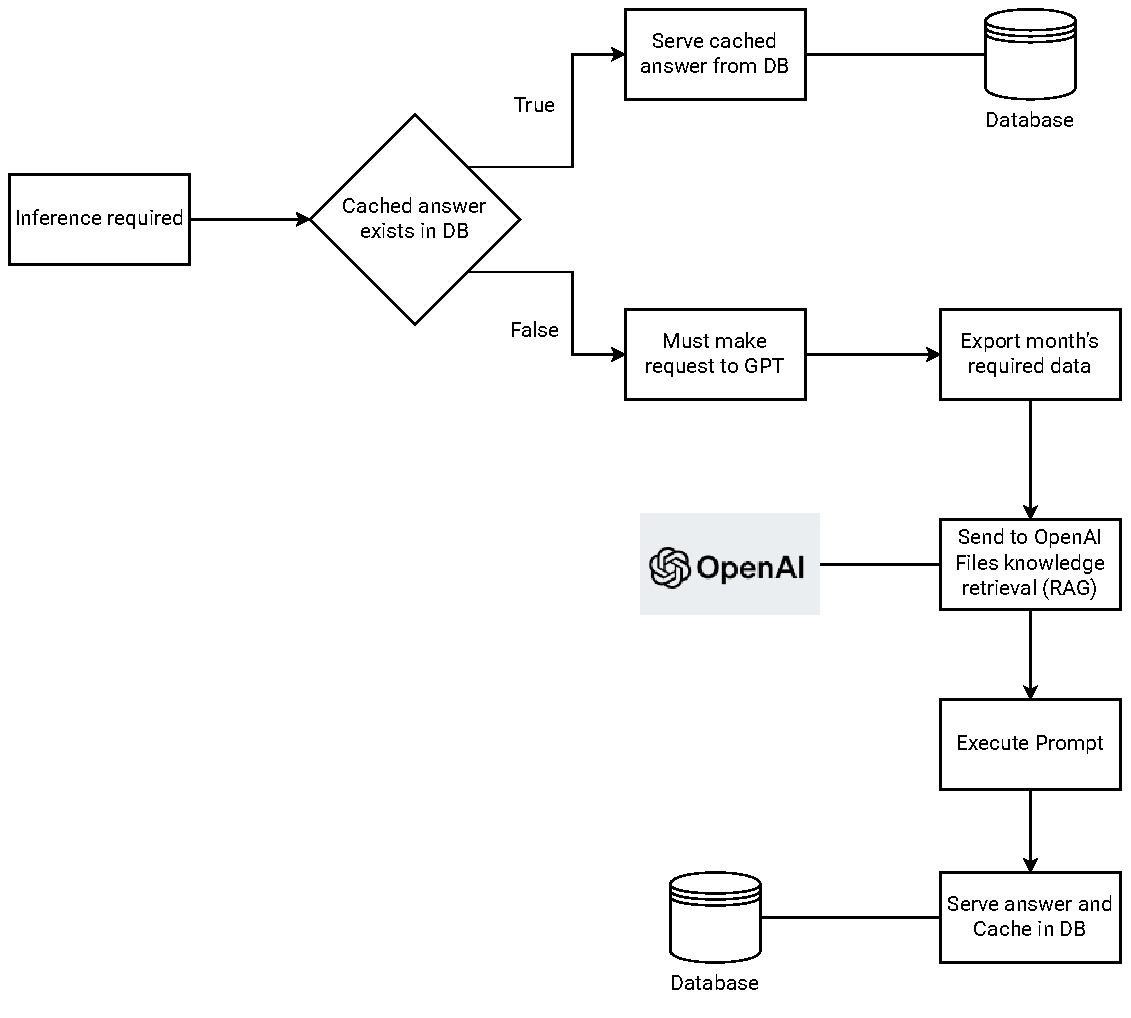
\includegraphics[width=\textwidth,height=\textheight,keepaspectratio]{../images/ai.pdf}
    \caption{AI Inference functionality Flow Chart}
    \label{fig:5}
    
\end{figure}


\begin{figure}
    
    \centering
    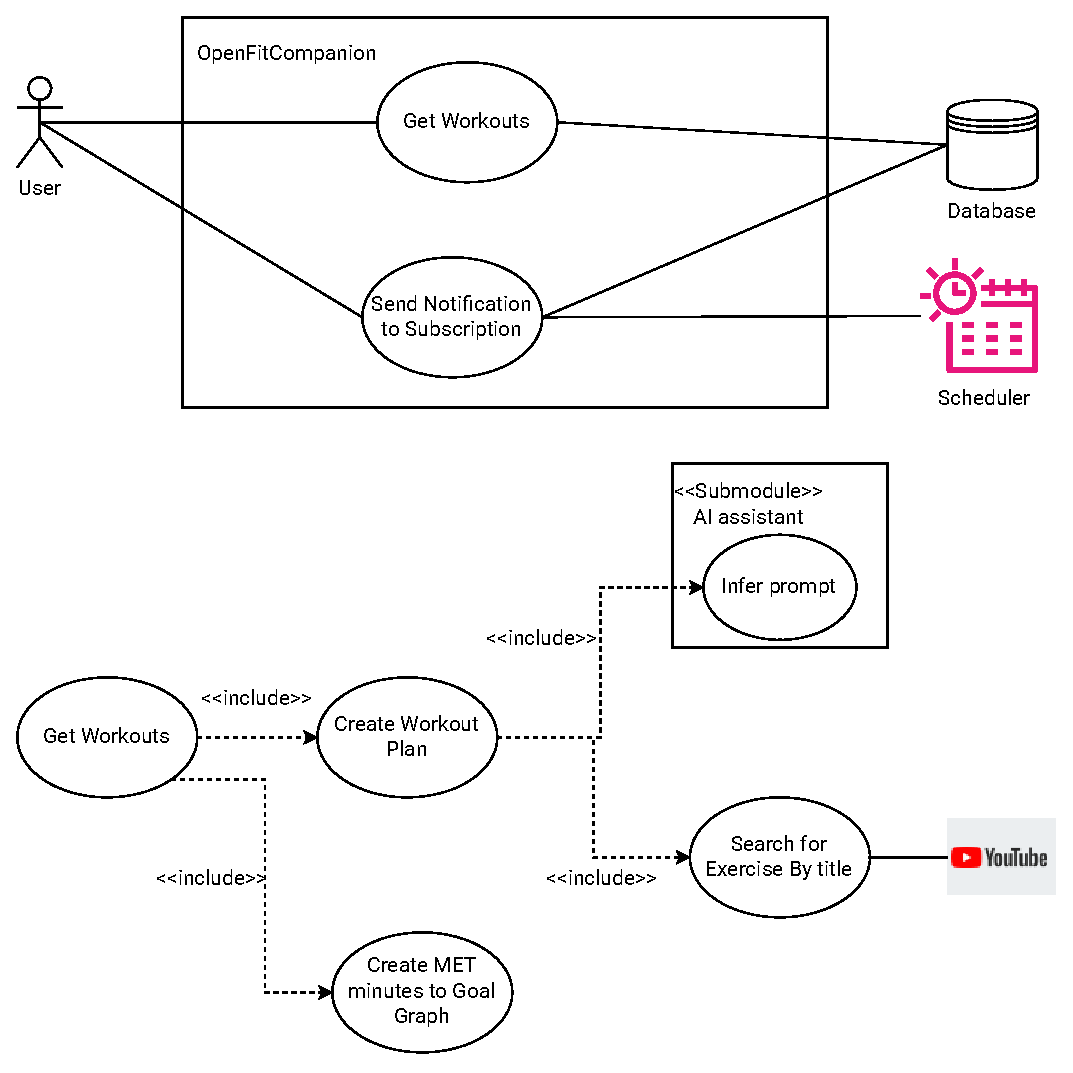
\includegraphics[width=\textwidth,height=\textheight,keepaspectratio]{../images/workouts.pdf}
    \caption{Activity plan use case UML diagram}
    \label{fig:6}
    
\end{figure}
\subsection{Non-Functional Requirements}
The following non-functional requirements for the system were gathered by inspecting general best practices and common sense. Represented as textual descriptions. 
\begin{itemize}
    \item Security: System must be secure and only allow access to the authenticated user. 
    \item Performance: UI must have low latency and feel snappy when used on a mobile network. 
    \item Usability: UI must be comfortably usable on mobile; openable as a native mobile app, supporting push notifications in the background (even if app is closed)
    \item Accessibility: UI must follow best practices supporting usage with assistive technologies such as screen readers, keyboard only etc
    \item Extensibility: The whole system should be easy to maintain and add new features; feature comprehensive logging and scale to add more providers
    \item Cost: Cost of running the service should be minimised while retaining required functionality.
\end{itemize}
\section{High-level overview}
\begin{figure}
    
    \centering
    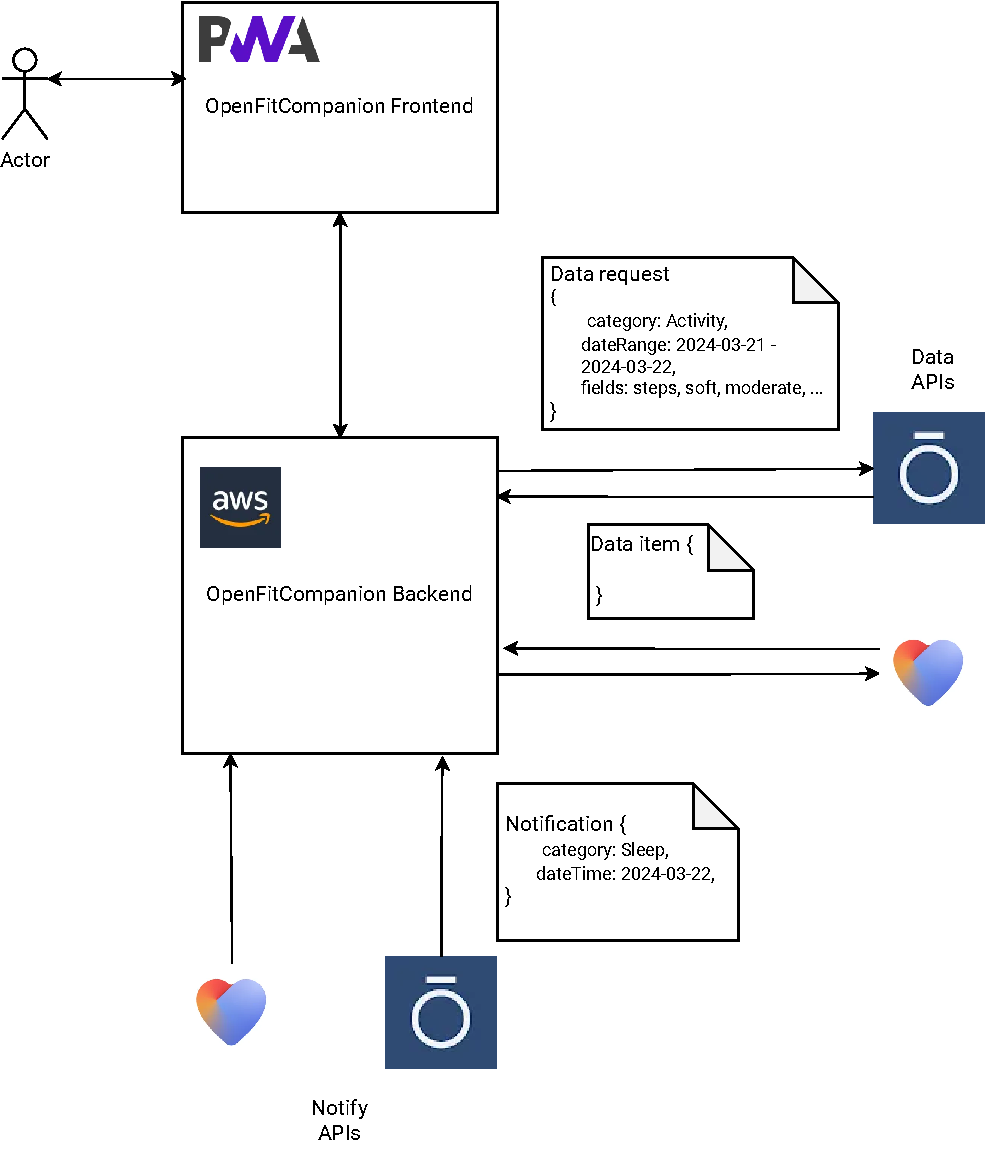
\includegraphics[width=\textwidth,height=\textheight,keepaspectratio]{../images/highLevel.pdf}
    \caption{High-Level architecture diagram}
    \label{fig:1}
    
\end{figure}
Overall, the architecture is considered event-driven. Computation only needs to happen in response to an external event. This is enabled by providers providing Webhook integrations. Essentially, the backend gets a notification from providers whenever there is new data available from them. The following is the diagram together with sample data exchanged: \ref{fig:1}

Cloud deployed backend service receives notifications from providers, containing information that allows atomic processing of that notification. It does not matter what other requests came before or if any are executing at the moment. 

In response to the notification, backend sends a request to Data APIs of providers, receiving an item(s) back and finally persisting it in a database for further purposes. 

Withings and Oura providers were integrated at the time of this report. However, the system can scale to many more providers. The only requirement for a provider is that they have Data API we can use. Even if a particular provider did not have a webhook (notification) service, we could re-sync with data APIs on regular schedule, like every 30 minutes. With the interval value being a trade-off between potentially more latency in syncing the data or wasted compute time when there are no updates. This would be quite costly if the system was publicly available service, as that scheduled request would be needed for each user. However, for our use case of self-deployed service, the cost would be negligible. However, there is still reliance on provider's API services to get the actual data from devices. System does not communicate with the smart devices directly via Bluetooth, there is an intermediate provider's system that data must be pass through. So, if a provider does not have such service, we can't integrate their devices into the system. However, all providers examined at least provided Google Fit integration, from which the data could be fetched instead. 

Ultimately, the data is transformed into useful information (insight) using using LLMs and classical algorithms. This is then presented to the user through the frontend. 
\begin{itemize}
    \item {Dashboard, contains a graph visualizing data from all devices, allowing for comparison and a brief overview of trends.}
    \item {Daily Report, containing a graph visualizing MET minutes completed this week and the goal MET minutes per week; Feedback on expected activity completion for that day and AI feedback for that day. Provides the user with information, allowing them to reflect on their day, seeing the progress towards fulfilling the weekly activity goal. A notification is sent to the user when such report is available. This constitutes Type 2 nudge, as it  engages user's conscious, reflective thinking to get them more motivated for physical activity tomorrow. However, there is also a component of Type 1 nudge with report notifications being opt-out rather than opt-in.}
    \item {Weekly Report, focusing more on consistency rather than absolute values and goal completions. Contains a graph visualizing deviation from the mean value of daily activity or sleep score. Same nudging as Daily Report.}
    \item {Activity plan, containing curated list of planned physical activities for the day, generated by AI. Also containing feedback about activity minutes done today. Similarly, it has type 1 nudging factor, being opt-out as well as Type 2 nudging, by notifying users at certain times when they should be doing exercises, and providing well-suited list of exercises, with description of benefits and video examples on how to perform them. This removes the need for user to plan their own workouts, removing decision paralysis. This imitates real-life coaching with a personal trainer, bringing benefits such as accountability and personalisation to users who may not be able to afford the real counterpart.}
\end{itemize}

\section{Back-end}
\subsection{Compute}
Because the system is event-driven, we can utilise serverless function as the main computing units in the backend; For AWS that is Lambda. Using Lambda is the most cost-effective option; it allows paying only for execution time down to milliseconds, free data out transfer to other AWS services. One disadvantage are cold starts, when a function is called for the first time in a while, it has increased latency due to some set-up, from my experiments it's around 400ms on average; and that happens for all Lambda functions, so if there is a chain of such functions called one after another, the latency will stack up and be quite noticeable. AWS provides the "Provisioned Concurrency", making sure that n functions are kept initialised and ready to respond at any time; however, it has a separate costing scheme similar to servers, whereby you pay by the second even if the function is never called. As per project aims, minimising cost is more important so the latency is something that is just tolerated.
\subsection{Persistance}
For persistance, DynamoDB is used. Because the service is meant to be used by a single user who is the owner of the self-deployed infrastructure, there is no need to identify to which user the row of data belongs to. Since DynamoDB, like most NoSQL databases does not support composite keys i.e keys that are made from 2+ fields; meaning that complexity has to be handled client-side. For example, using field1 and field2 as PK involves having single field PK and using something like "field1\_\_DELIM\_\_field2" as the value, and checking that delimiting string does not form naturally (which is unlikely) from fields values to ensure uniqueness. To improve robustness a simple client-side schema that relies on Typescript classes was designed. Primary key schema is derived by considering access patterns to that table. For example, with health data: \ref{fig:schema}, the typical functionality is querying a certain data type (sleep, activity) originating from a certain provider between a range of dates; using the key schema in the diagram, this typical request can be handled efficiently by setting composite partition key and using DynamoDB range query of BETWEEN with no need for expensive client-side filtering. 
\begin{figure}
    
    \centering
    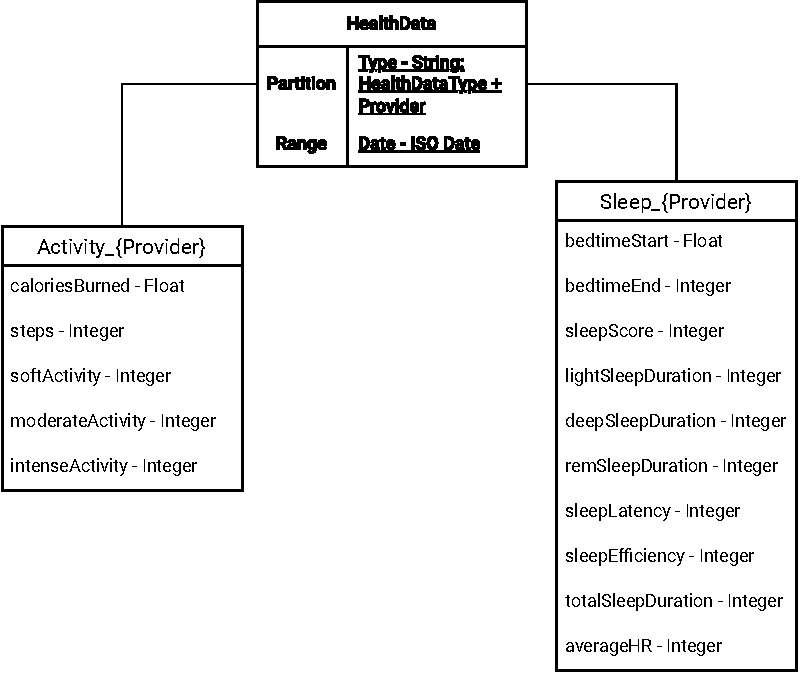
\includegraphics[width=\textwidth,height=\textheight,keepaspectratio]{../images/dataSchema.pdf}
    \caption{HealthData Table client-side Schema}
    \label{fig:schema}
    
\end{figure}
\subsection{Unifying}
Although data from all devices is stored and can be viewed separately, for many purposes such as AI insights there needs to be a single row for each date that is treated as ground-truth. For this, measurements from all devices are averaged out and stored under "Unified" Provider. 
\subsection{Architecture}
\begin{figure}
    
    \centering
    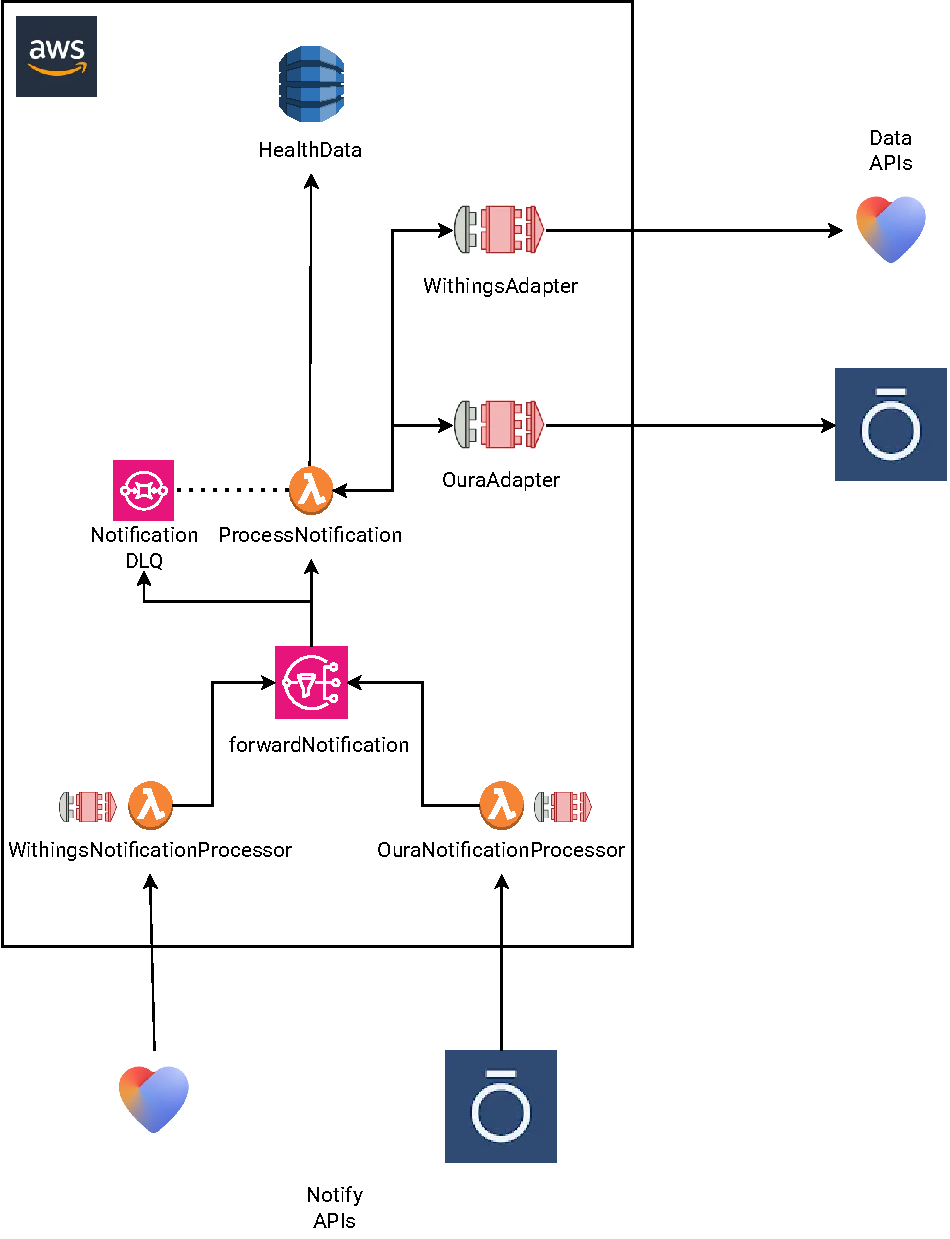
\includegraphics[width=\textwidth,height=\textheight,keepaspectratio]{../images/backend.pdf}
    \caption{Backend Architecture Diagram}
    \label{fig:backend}
    
\end{figure}
Breaking down purpose of each component in \ref{fig:backend}: (Note: Some of the backend components are in, as to not clutter the diagram and semantically they are more about interaction with the frontend.)
\begin{itemize}
    \item {WithingsAdapter \& OuraAdapter: Software classes for abstracting complexities of interfacing with external providers - Adapter pattern. Different providers require different: formats for the request, authentication, attribute unit conversions, etc. These adapters handle such intricacies while providing an easy, consistent interface.}
    \item {WithingsNotificationProcessor \& OuraNotificationProcessor Lambdas: Providers send HTTP request to a callback url specified when creating a webhook. These functions are for handling those notification HTTP requests, extracting relevant information and passing it to the SNS. There are 2 of them because notifications from different providers require different processing. Uses adapter components.}
    \item {ForwardNotification SNS \& NotificationDLQ: Decouples the system as Lambdas directly invoking other Lambdas is a bad practice: worse observability, harder exception handling, etc. SNS is preferable to SQS, because it fits in a serverless architecture better and costs less due to it being a push model rather than SQS polling. Failed requests from SNS are sent to the Dead-Letter-Queue and saved so that they can be re-processed later; this allows the system to tolerate external services faults.}
    \item {ProcessNotifcation Lambda: Triggered by notification, uses adapters to request data item(s) from providers and stores in the database.}
\end{itemize}

\section{Front-end}
\subsection{UI}
\subsection{Notifying}
\subsection{Reporting}

TODO: Do this chapter
